\renewcommand{\theequation}{\theenumi}
\begin{enumerate}[label=\thesection.\arabic*.,ref=\thesection.\theenumi]
\numberwithin{equation}{enumi}

\item Substituting \ref{eq:pointd} in \ref{eq:centr} we get
\begin{align}
\implies \vec{O}=\frac{\vec{B}+\vec{C}+\vec{A}}{3}
\end{align}

The following code plots figure \ref{fig:median}
\begin{lstlisting}
codes/line/median/median.py
\end{lstlisting}
\begin{figure}[!ht]
\centering
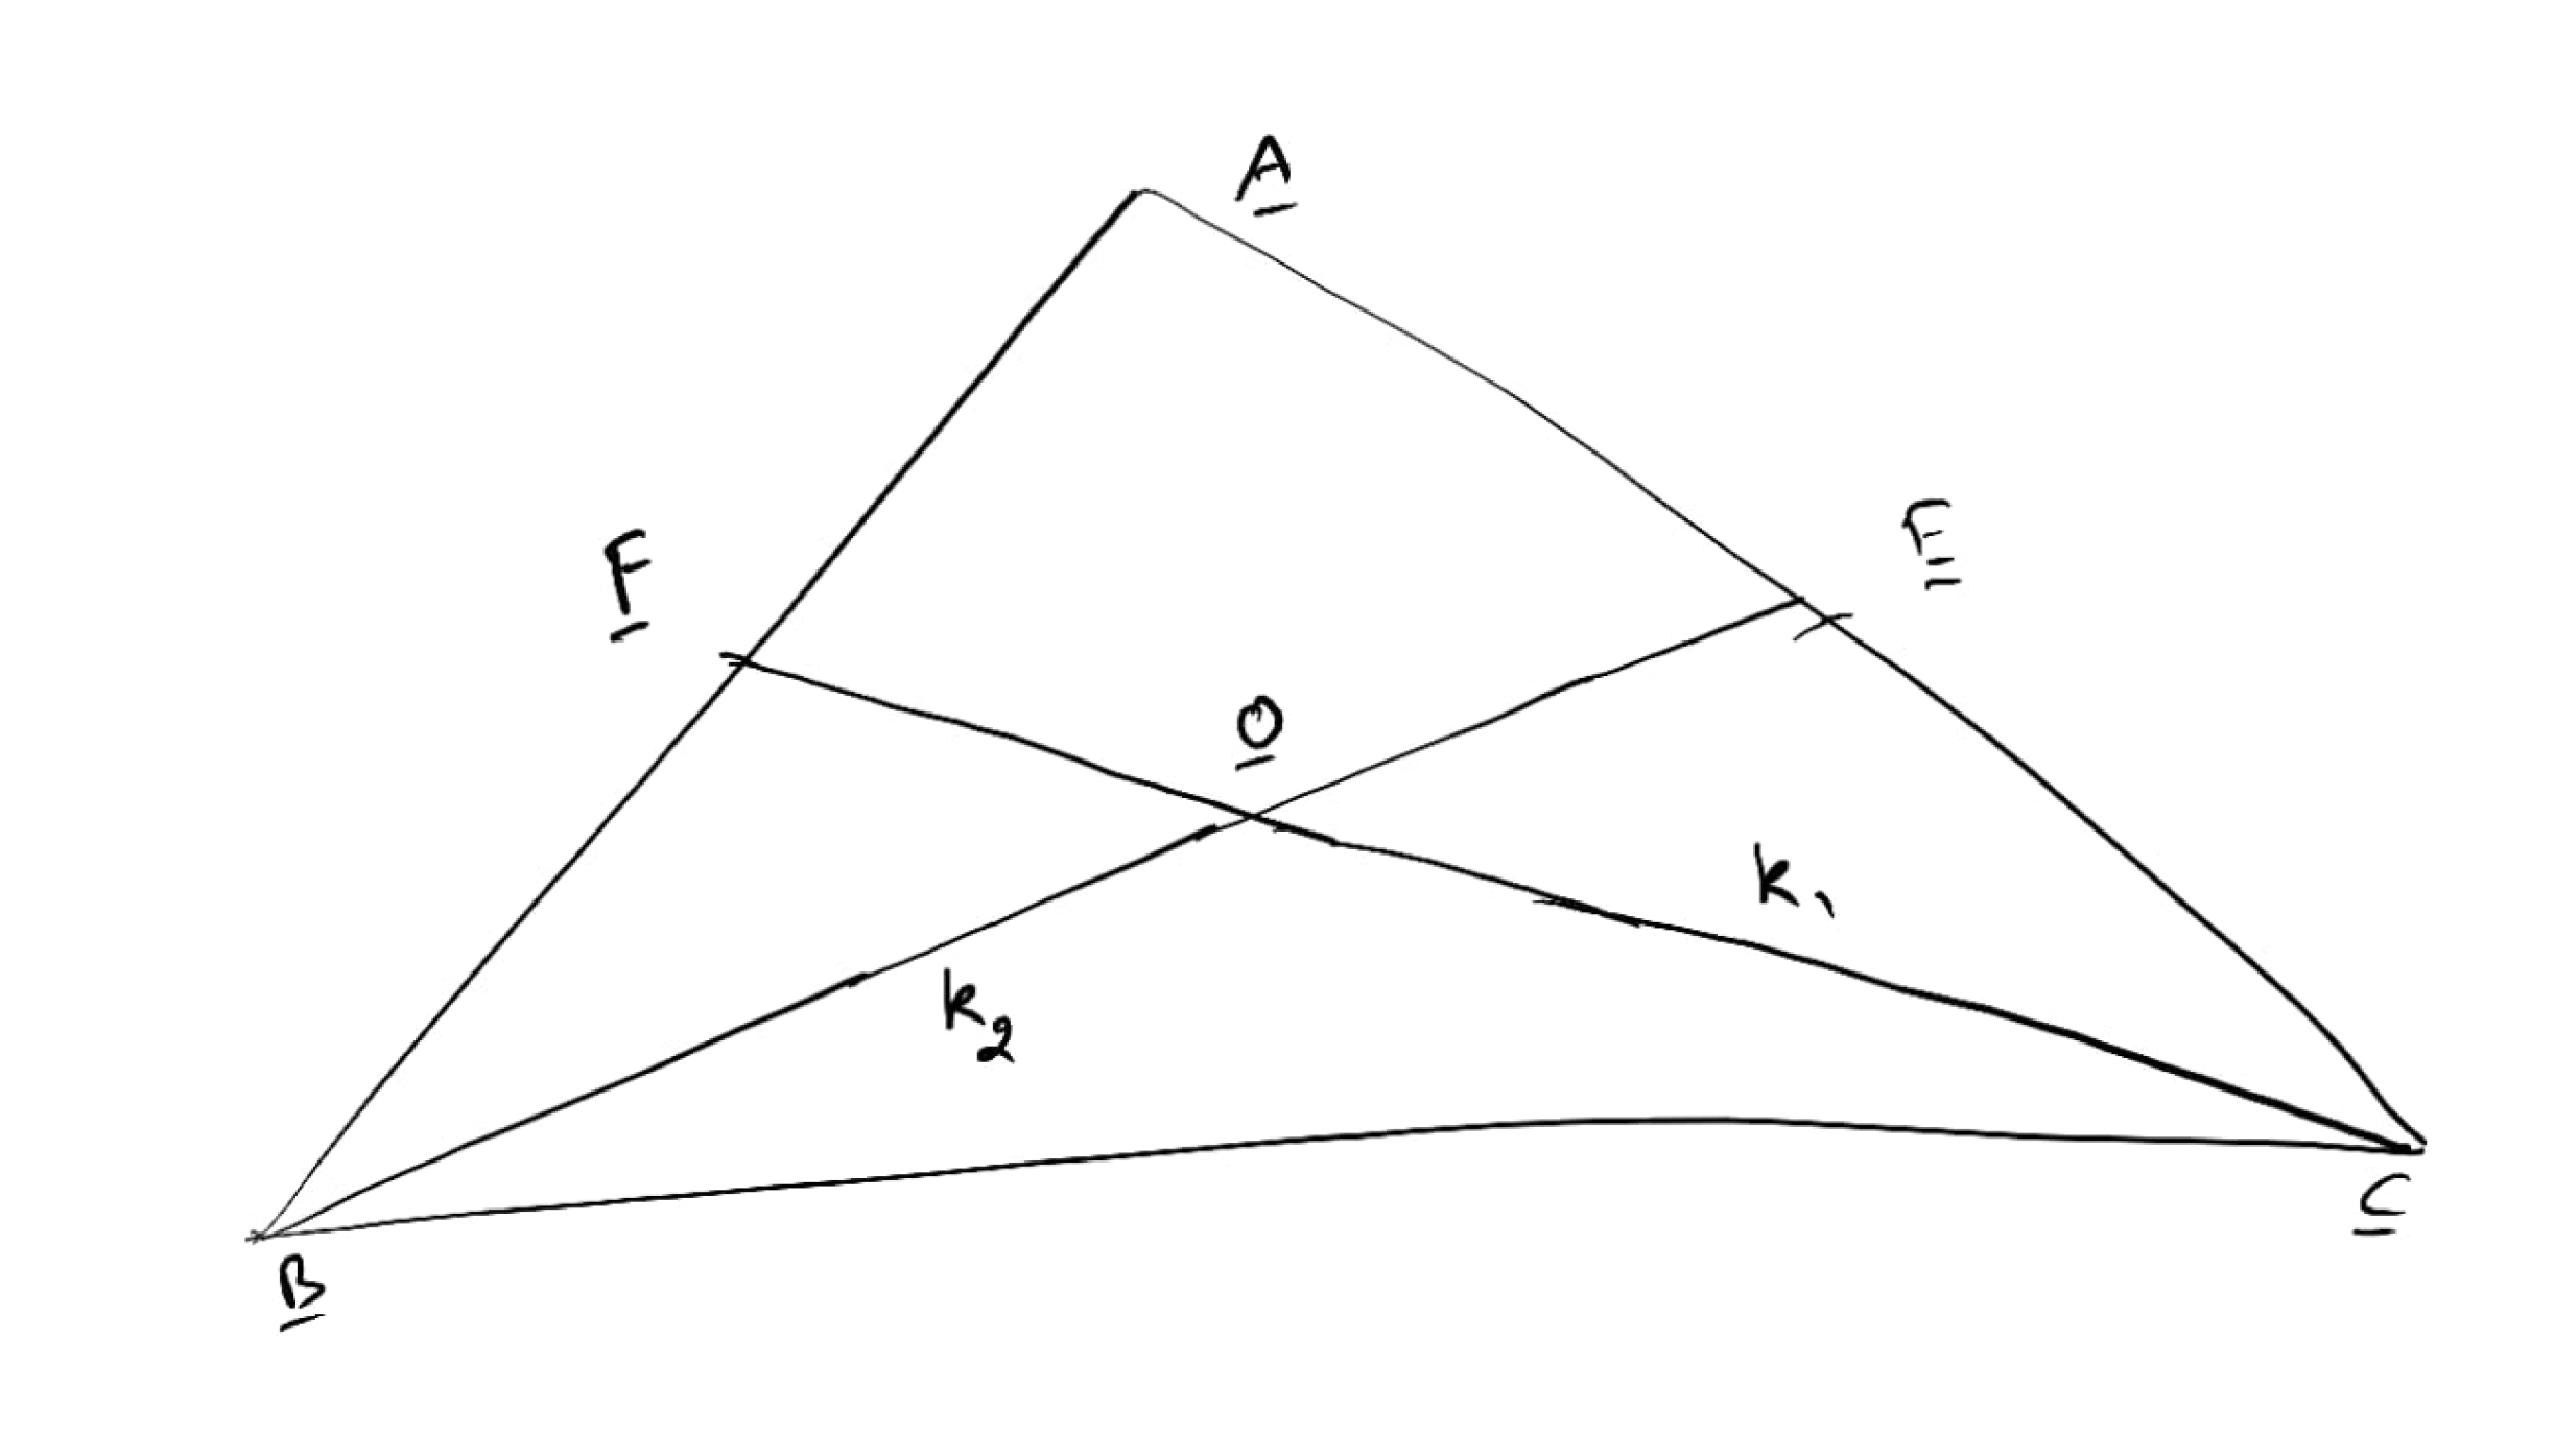
\includegraphics[width=\columnwidth]{./codes/line/median/pyfigs/median.eps}
\caption{Triangle ABC with centroid O}
\label{fig:median}
\end{figure}

\end{enumerate}
